% Thanks to Kevin D. McGrath for the presentation template.
\documentclass[xcolor={dvipsnames,svgnames},hyperref=dvips]{beamer}

% Packages.
\usepackage{amsmath}
\usepackage{color}
\usepackage{graphicx}

% Hyperlinks.
\def\name{Wade Cline}
\hypersetup{
  colorlinks = true,
  citecolor = black,
  linkcolor = black,
  urlcolor = black,
  pdfauthor = {\name},
  pdftitle = {X.509},
  pdfsubject = {X.509},
  pdfpagemode = UseNone
}

% ???
\usetheme[hideothersubsections]{Hannover}
\usecolortheme{sidebartab}

% Presentation metadata.
\title[X.509 Introduction]{A Brief Introduction to SSL/TLS X.509 Certificates}
\author{Wade Cline}
\date{April 8th, 2017}

\AtBeginSection[]
{
  \begin{frame}<beamer>{Outline}
    \tableofcontents[currentsection]
  \end{frame}
}
%\AtBeginSubsection[]
%{
%  \begin{frame}<beamer>{Outline}
%    % \transwipe
%    \tableofcontents[currentsection,currentsubsection]
%  \end{frame}
%}

\begin{document}

% Title.
\begin{frame}
  \titlepage
\end{frame}

% Table of Contents.
\begin{frame}{Outline}
  % \transwipe
  \tableofcontents
  % You might wish to add the option [pausesections]
\end{frame}

\section{Primer}
	\begin{frame}
		\frametitle{Public/Private Key Cryptography}
		\begin{itemize}
		\item \textit{Public} and \textit{Private} key pairs.
		\item \textit{Share} public keys.  \textit{Hide} private keys.
		\item Simple user: \textit{Many} public keys, \textit{one} private key.
		\item Public key to \textit{send}, private key to \textit{recieve}.
		\end{itemize}
	\end{frame}

	\begin{frame}
		\frametitle{Network Layers}
		\begin{itemize}
		\item Five\footnote{No one cares about OSI's 7-layer model.} network \textit{layers}.
			\begin{itemize}
			\item Application Layer (HTTP, IRC, IMAP, SSH, Git, \&c.)
			\item \textbf{Transport Layer} (TCP/UDP).
			\item \textbf{Network Layer} (IPv4/IPv6).
			\item Link Layer (WiFi, Ethernet).
			\item Physical Layer.
			\end{itemize}
		\end{itemize}
	\end{frame}

	\begin{frame}
		\frametitle{TLS/SSL}
		\begin{itemize}
		\item Naming sucks.
			\begin{itemize}
			\item SSL (Secure Sockets Layer) -- old.
			\item TLS (Transport Layer Security) -- new.
			\end{itemize}
		\item Encrypt TCP/IP connections.
		\item Use \textit{X.509} certificates for \textit{authentication} and \textit{authorization}.
		\item Various implementations:
			\begin{itemize}
			\item \texttt{openssl}
			\item \texttt{gnutls}
			\item \texttt{libressl}
			\end{itemize}
		\end{itemize}
	\end{frame}

\section{X.509}
\subsection{About}
	\begin{frame}
		\frametitle{What does X.509 mean?}
		\begin{itemize}
		\item Created in association with X.500 standard.
		\item Based on ASN.1.
		\item Defined by the International Telecommunications Union (ITU-T).
		\item Artists depiction: \\
			\center\includegraphics[scale=0.27]{wtfsoup.ps}
		\end{itemize}
	\end{frame}

	\begin{frame}
		\frametitle{Overview}
		\begin{itemize}
		\item The \textit{public key} of TLS.
		\item Called \textit{certificate}.
		\item \textit{Share} the \textbf{certificate}.  \textit{Hide} the key.
		\item Certificate Authorities!
		\item Confusing terminology!
		\end{itemize}
	\end{frame}

	\begin{frame}
		\frametitle{Certificate Authorities (CAs)}
		\begin{itemize}
		\item \textit{Hierarchy} of trust.
		\item \textit{Root CA} at top, then \textit{Intermediate CAs}.
		\item Root certificate (Root CA) $\rightarrow$ Intermediate certificate(s)\footnote{Zero or more.} (Intermediate CA(s)) $\rightarrow$ Leaf\footnote{Do these even have a formal name?} Certificate\footnote{Or just use the root certificate as a leaf certificate.  That's cool, too.} (You)
		\item Path is a certificate \textit{chain of trust}.
		\end{itemize}
	\end{frame}

	\begin{frame}
		\frametitle{Artist's Depiction}
		\center\includegraphics[scale=0.5]{chainoftrustpt1.ps}
	\end{frame}

	\begin{frame}
		\frametitle{Artist's Depiction pt2}
		\center\includegraphics[scale=0.18]{chainoftrustpt2.ps}
	\end{frame}

	\begin{frame}
		\frametitle{Terminology}
		\begin{itemize}
		\item Issuer \& Subject.
			\begin{itemize}
			\item Subject \textit{recieves} certificate from issuer.
			\item Subject usually \textit{you}.
			\item \textbf{Bloated} fields consist of \textbf{beaurcratic crap}:
				\begin{itemize}
				\item Country Name $\leftarrow$ One world, man.
				\item State or Provience Name $\leftarrow$ Cascadia, obvs.
				\item Locality Name $\leftarrow$ wtf?
				\item Organization Name $\leftarrow$ "A Dude".
				\item Organization Unit Name $\leftarrow$ W.T.F.?
				\item \textbf{Common Name} $\leftarrow$ Only sane field (usually your FQDN).
				\item E-mail Address $\leftarrow$ For spambots.
				\end{itemize}
			\item CAs \textit{may} omit fields.
			\end{itemize}
		\item Client and Server certificates.
			\begin{itemize}
			\item Client certificates rare, often not used on home browsers.
			\end{itemize}
		\end{itemize}
	\end{frame}

\subsection{The PKI}
	\begin{frame}
		\frametitle{About}
		\begin{itemize}
		\item PKI (Public Key Infrastructure).
		\item Manages certificates.
		\item Many PKIs.
		\item Usually browser's implementation.
		\end{itemize}
	\end{frame}

	\begin{frame}
		\frametitle{Viewing}
		\begin{itemize}
		\item \texttt{/usr/share/ca-certificates/}
		\item Subdirectories possible.
		\item Let's have a trust survey!
			\begin{itemize}
			\item Unique \textbf{Organization} field.
			\end{itemize}
		\end{itemize}
	\end{frame}

	% BEGIN ROOT CA SPAM.
	\begin{frame}
		\begin{itemize}
		\item Subject: C=ES, CN=Autoridad de Certificacion Firmaprofesional CIF A62634068
		\item Subject: C=EU, L=Madrid (see current address at www.camerfirma.com/address)/serialNumber=A82743287, O=AC Camerfirma S.A., CN=Global Chambersign Root - 2008
		\item Subject: C=EU, O=AC Camerfirma SA CIF A82743287, OU=http://www.chambersign.org, CN=Chambers of Commerce Root
		\item Subject: CN=ACCVRAIZ1, OU=PKIACCV, O=ACCV, C=ES
		\item Subject: C=EE, O=AS Sertifitseerimiskeskus, CN=EE Certification Centre Root CA/emailAddress=pki@sk.ee
		\end{itemize}
	\end{frame}
	\begin{frame}
		\begin{itemize}
		\item Subject: C=IT, L=Milan, O=Actalis S.p.A./03358520967, CN=Actalis Authentication Root CA
		\item Subject: C=SE, O=AddTrust AB, OU=AddTrust TTP Network, CN=AddTrust Public CA Root
		\item Subject: C=US, O=AffirmTrust, CN=AffirmTrust Premium ECC
		\item Subject: C=ES, O=Agencia Catalana de Certificacio (NIF Q-0801176-I), OU=Serveis Publics de Certificacio, OU=Vegeu https://www.catcert.net/verarrel (c)03, OU=Jerarquia Entitats de Certificacio Catalanes, CN=EC-ACC
		\item Subject: CN=Atos TrustedRoot 2011, O=Atos, C=DE
		\end{itemize}
	\end{frame}
	\begin{frame}
		\begin{itemize}
		\item Subject: C=IE, O=Baltimore, OU=CyberTrust, CN=Baltimore CyberTrust Root
		\item Subject: C=NO, O=Buypass AS-983163327, CN=Buypass Class 2 Root CA
		\item Subject: C=CN, O=CNNIC, CN=CNNIC ROOT
		\item Subject: C=GB, ST=Greater Manchester, L=Salford, O=COMODO CA Limited, CN=COMODO RSA Certification Authority
		\item Subject: C=FR, O=Certinomis, OU=0002 433998903, CN=Certinomis - Root CA
		\end{itemize}
	\end{frame}
	\begin{frame}
		\begin{itemize}
		\item Subject: C=FR, O=Certplus, CN=Class 2 Primary CA
		\item Subject: C=CN, O=China Financial Certification Authority, CN=CFCA EV ROOT
		\item Subject: C=CN, O=China Internet Network Information Center, CN=China Internet Network Information Center EV Certificates Root
		\item Subject: C=TW, O=Chunghwa Telecom Co., Ltd., OU=ePKI Root Certification Authority
		\item Subject: CN=ComSign CA, O=ComSign, C=IL
		\end{itemize}
	\end{frame}
	\begin{frame}
		\begin{itemize}
		\item Subject: C=GB, ST=Greater Manchester, L=Salford, O=Comodo CA Limited, CN=AAA Certificate Services
		\item Subject: O=Cybertrust, Inc, CN=Cybertrust Global Root
		\item Subject: C=DE, O=D-Trust GmbH, CN=D-TRUST Root Class 3 CA 2 2009
		\item Subject: C=DE, O=Deutsche Telekom AG, OU=T-TeleSec Trust Center, CN=Deutsche Telekom Root CA 2
		\item Subject: C=DE, O=Deutscher Sparkassen Verlag GmbH, OU=S-TRUST Certification Services, CN=S-TRUST Universal Root CA
		\end{itemize}
	\end{frame}
	\begin{frame}
		\begin{itemize}
		\item Subject: C=FR, O=Dhimyotis, CN=Certigna
		\item Subject: C=US, O=DigiCert Inc, OU=www.digicert.com, CN=DigiCert Assured ID Root G3
		\item Subject: C=US, O=Digital Signature Trust, OU=DST ACES, CN=DST ACES CA X6
		\item Subject: O=Digital Signature Trust Co., CN=DST Root CA X3
		\item Subject: C=SK, L=Bratislava, O=Disig a.s., CN=CA Disig Root R2
		\end{itemize}
	\end{frame}
	\begin{frame}
		\begin{itemize}
		\item Subject: C=TR, L=Ankara, O=E-Tu\textbackslash xC4\textbackslash x9Fra EBG Bili\textbackslash xC5\textbackslash x9Fim Teknolojileri ve Hizmetleri A.\textbackslash xC5\textbackslash x9E., OU=E-Tugra Sertifikasyon Merkezi, CN=E-Tugra Certification Authority
		\item Subject: CN=ACEDICOM Root, OU=PKI, O=EDICOM, C=ES
		\item Subject: C=US, O=Entrust, Inc., OU=See www.entrust.net/legal-terms, OU=(c) 2009 Entrust, Inc. - for authorized use only, CN=Entrust Root Certification Authority - G2
		\item Subject: O=Entrust.net, OU=www.entrust.net/CPS\_2048 incorp. by ref. (limits liab.), OU=(c) 1999 Entrust.net Limited, CN=Entrust.net Certification Authority (2048)
		\item Subject: C=ES, O=Generalitat Valenciana, OU=PKIGVA, CN=Root CA Generalitat Valenciana
		\end{itemize}
	\end{frame}
	\begin{frame}
		\begin{itemize}
		\item Subject: C=US, O=GeoTrust Inc., CN=GeoTrust Primary Certification Authority
		\item Subject: OU=GlobalSign Root CA - R3, O=GlobalSign, CN=GlobalSign
		\item Subject: C=BE, O=GlobalSign nv-sa, OU=Root CA, CN=GlobalSign Root CA
		\item Subject: C=US, ST=Arizona, L=Scottsdale, O=GoDaddy.com, Inc., CN=Go Daddy Root Certificate Authority - G2
		\item Subject: C=TW, O=Government Root Certification Authority
		\end{itemize}
	\end{frame}
	\begin{frame}
		\begin{itemize}
		\item Subject: C=GR, L=Athens, O=Hellenic Academic and Research Institutions Cert. Authority, CN=Hellenic Academic and Research Institutions RootCA 2015
		\item Subject: C=HK, O=Hongkong Post, CN=Hongkong Post Root CA 1
		\item Subject: C=ES, O=IZENPE S.A., CN=Izenpe.com
		\item Subject: C=US, O=IdenTrust, CN=IdenTrust Public Sector Root CA 1
		\item Subject: C=US, O=Internet Security Research Group, CN=ISRG Root X1
		\end{itemize}
	\end{frame}
	\begin{frame}
		\begin{itemize}
		\item Subject: C=JP, O=Japan Certification Services, Inc., CN=SecureSign RootCA11
		\item Subject: C=JP, O=Japanese Government, OU=ApplicationCA
		\item Subject: C=PL, O=Krajowa Izba Rozliczeniowa S.A., CN=SZAFIR ROOT CA2
		\item Subject: C=HU, L=Budapest, O=Microsec Ltd., OU=e-Szigno CA, CN=Microsec e-Szigno Root CA
		\item Subject: C=HU, L=Budapest, O=NetLock Kft., OU=Tan\textbackslash xC3\textbackslash xBAs\textbackslash xC3\textbackslash xADtv\textbackslash xC3\textbackslash xA1nykiad\textbackslash xC3\textbackslash xB3k (Certification Services), CN=NetLock Arany (Class Gold) F\textbackslash xC5\textbackslash x91tan\textbackslash xC3\textbackslash xBAs\textbackslash xC3\textbackslash xADtv\textbackslash xC3\textbackslash xA1ny
		\end{itemize}
	\end{frame}
	\begin{frame}
		\begin{itemize}
		\item Subject: C=US, O=Network Solutions L.L.C., CN=Network Solutions Certificate Authority
		\item Subject: C=FR, O=OpenTrust, CN=OpenTrust Root CA G2
		\item Subject: C=BM, O=QuoVadis Limited, CN=QuoVadis Root CA 3 G3
		\item Subject: O=RSA Security Inc, OU=RSA Security 2048 V3
		\item Subject: C=JP, O=SECOM Trust Systems CO.,LTD., OU=Security Communication RootCA2
		\end{itemize}
	\end{frame}
	\begin{frame}
		\begin{itemize}
		\item Subject: C=JP, O=SECOM Trust.net, OU=Security Communication RootCA1
		\item Subject: C=US, O=SecureTrust Corporation, CN=Secure Global CA
		\item Subject: emailAddress=contacto@procert.net.ve, L=Chacao, ST=Miranda, OU=Proveedor de Certificados PROCERT, O=Sistema Nacional de Certificacion Electronica, C=VE, CN=PSCProcert
		\item Subject: C=CO, O=Sociedad Cameral de Certificaci\textbackslash xC3\textbackslash xB3n Digital - Certic\textbackslash xC3\textbackslash xA1mara S.A., CN=AC Ra\textbackslash xC3\textbackslash xADz Certic\textbackslash xC3\textbackslash xA1mara S.A.
		\item Subject: C=FI, O=Sonera, CN=Sonera Class2 CA
		\end{itemize}
	\end{frame}
	\begin{frame}
		\begin{itemize}
		\item Subject: C=NL, O=Staat der Nederlanden, CN=Staat der Nederlanden EV Root CA
		\item Subject: C=US, ST=Arizona, L=Scottsdale, O=Starfield Technologies, Inc., CN=Starfield Root Certificate Authority - G2
		\item Subject: C=CH, O=SwissSign AG, CN=SwissSign Platinum CA - G2
		\item Subject: C=ch, O=Swisscom, OU=Digital Certificate Services, CN=Swisscom Root CA 2
		\item Subject: C=DE, O=T-Systems Enterprise Services GmbH, OU=T-Systems Trust Center, CN=T-TeleSec GlobalRoot Class 2
		\end{itemize}
	\end{frame}
	\begin{frame}
		\begin{itemize}
		\item Subject: C=TW, O=TAIWAN-CA, OU=Root CA, CN=TWCA Global Root CA
		\item Subject: C=DE, O=TC TrustCenter GmbH, OU=TC TrustCenter Class 3 CA, CN=TC TrustCenter Class 3 CA II
		\item Subject: C=TR, L=Ankara, O=T\textbackslash xC3\textbackslash x9CRKTRUST Bilgi \textbackslash xC4\textbackslash xB0leti\textbackslash xC5\textbackslash x9Fim ve Bili\textbackslash xC5\textbackslash x9Fim G\textbackslash xC3\textbackslash xBCvenli\textbackslash xC4\textbackslash x9Fi Hizmetleri A.\textbackslash xC5\textbackslash x9E., CN=T\textbackslash xC3\textbackslash x9CRKTRUST Elektronik Sertifika Hizmet Sa\textbackslash xC4\textbackslash x9Flay\textbackslash xC4\textbackslash xB1c\textbackslash xC4\textbackslash xB1s\textbackslash xC4\textbackslash xB1 H5
		\item Subject: CN=T\textbackslash xC3\textbackslash x9CRKTRUST Elektronik Sertifika Hizmet Sa\textbackslash xC4\textbackslash x9Flay\textbackslash xC4\textbackslash xB1c\textbackslash xC4\textbackslash xB1s\textbackslash xC4\textbackslash xB1, C=TR, L=Ankara, O=T\textbackslash xC3\textbackslash x9CRKTRUST Bilgi \textbackslash xC4\textbackslash xB0leti\textbackslash xC5\textbackslash x9Fim ve Bili\textbackslash xC5\textbackslash x9Fim G\textbackslash xC3\textbackslash xBCvenli\textbackslash xC4\textbackslash x9Fi Hizmetleri A.\textbackslash xC5\textbackslash x9E. (c) Aral\textbackslash xC4\textbackslash xB1k 2007
		\item Subject: C=TR, L=Gebze - Kocaeli, O=T\textbackslash xC3\textbackslash xBCrkiye Bilimsel ve Teknolojik Ara\textbackslash xC5\textbackslash x9Ft\textbackslash xC4\textbackslash xB1rma Kurumu - T\textbackslash xC3\textbackslash x9CB\textbackslash xC4\textbackslash xB0TAK, OU=Ulusal Elektronik ve Kriptoloji Ara\textbackslash xC5\textbackslash x9Ft\textbackslash xC4\textbackslash xB1rma Enstit\textbackslash xC3\textbackslash xBCs\textbackslash xC3\textbackslash xBC - UEKAE, OU=Kamu Sertifikasyon Merkezi, CN=T\textbackslash xC3\textbackslash x9CB\textbackslash xC4\textbackslash xB0TAK UEKAE K\textbackslash xC3\textbackslash xB6k Sertifika Hizmet Sa\textbackslash xC4\textbackslash x9Flay\textbackslash xC4\textbackslash xB1c\textbackslash xC4\textbackslash xB1s\textbackslash xC4\textbackslash xB1 - S\textbackslash xC3\textbackslash xBCr\textbackslash xC3\textbackslash xBCm 3
		\end{itemize}
	\end{frame}
	\begin{frame}
		\begin{itemize}
		\item Subject: O=TeliaSonera, CN=TeliaSonera Root CA v1
		\item Subject: C=US, O=The Go Daddy Group, Inc., OU=Go Daddy Class 2 Certification Authority
		\item Subject: C=US, ST=New Jersey, L=Jersey City, O=The USERTRUST Network, CN=USERTrust ECC Certification Authority
		\item Subject: C=GB, O=Trustis Limited, OU=Trustis FPS Root CA
		\item Subject: C=PL, O=Unizeto Sp. z o.o., CN=Certum CA
		\end{itemize}
	\end{frame}
	\begin{frame}
		\begin{itemize}
		\item Subject: C=PL, O=Unizeto Technologies S.A., OU=Certum Certification Authority, CN=Certum Trusted Network CA 2
		\item Subject: C=US, O=VISA, OU=Visa International Service Association, CN=Visa eCommerce Root
		\item Subject: C=US, O=VeriSign, Inc., OU=VeriSign Trust Network, OU=(c) 1999 VeriSign, Inc. - For authorized use only, CN=VeriSign Class 3 Public Primary Certification Authority - G3
		\item Subject: C=CH, O=WISeKey, OU=OISTE Foundation Endorsed, CN=OISTE WISeKey Global Root GB CA
		\item Subject: C=US, O=Wells Fargo WellsSecure, OU=Wells Fargo Bank NA, CN=WellsSecure Public Root Certificate Authority
		\end{itemize}
	\end{frame}
	\begin{frame}
		\begin{itemize}
		\item Subject: C=CN, O=WoSign CA Limited, CN=Certification Authority of WoSign G2
		\item Subject: C=US, OU=www.xrampsecurity.com, O=XRamp Security Services Inc, CN=XRamp Global Certification Authority
		\item Subject: C=RO, O=certSIGN, OU=certSIGN ROOT CA
		\item Subject: C=US, O=thawte, Inc., OU=Certification Services Division, OU=(c) 2006 thawte, Inc. - For authorized use only, CN=thawte Primary Root CA
		\end{itemize}
	\end{frame}
	% END ROOT CA SPAM.

	\begin{frame}
		\begin{itemize}
		\item Listed root CAs, not intermediate CAs.
		\item "I trust browser vendors".
		\begin{itemize}
			\item Not unreasonable.
		\end{itemize}
		\item Might not always trust.
		\item Why deal with PKI ha\$\$le?
		\end{itemize}
	\end{frame}

	\begin{frame}
		\center\includegraphics[scale=0.20]{darksidecerts.ps}
	\end{frame}

\section{OpenSSL}
\subsection{Basic Usage}
	\begin{frame}
		\frametitle{Subcommands}
		\begin{itemize}
			\item \texttt{s\_client} -- Connect to SSL/TLS service.
			\item \texttt{x\_509} -- Mostly reading certificates.
			\item \texttt{genrsa} -- Generate private RSA key.
			\item \texttt{req} -- Generate Certificate Signing Requests (CSRs).
			\item \textcolor{gray}{\texttt{ca} -- Sign CSRs.}
			\item \textcolor{gray}{\texttt{verify} -- Test certificate authentication.}
			\item[]
			\item \texttt{man} pages no \texttt{openssl} prefix (ex: \texttt{man x509}).
		\end{itemize}
	\end{frame}

	\begin{frame}
		\frametitle{Get Server Cert.}
		\begin{itemize}
			\item Use \texttt{s\_client}.
			\item Example for \texttt{google.com}: '\texttt{openssl s\_client -showcerts -connect google.com:443}'.
			\begin{itemize}
				\item \texttt{-showcerts} show intermediate certs (else only ``leaf'' cert).
				\item \texttt{-connect} \texttt{<address>:<port>}.
				\item SIGINT to close connection (\texttt{\textasciicircum C}).
				\item Yank cert(s) via X clipboard (or ugly \texttt{sed}).
			\end{itemize}
		\end{itemize}
	\end{frame}
	\begin{frame}
		\center\includegraphics[scale=0.4]{pemcert.ps}
	\end{frame}

	\begin{frame}
		\frametitle{View Cert.}
		\begin{itemize}
			\item Two formats: DER and PEM.
			\begin{itemize}
				\item DER $\approx$ GPG (binary)
				\item PEM $\approx$ ASC (text)
			\end{itemize}
			\item Use \texttt{x509}.
			\item Example: \texttt{openssl x509 -in cert.pem -text}
			\begin{itemize}
				\item \texttt{-in <file>} cert. to read.
				\item \texttt{-text} output cert's text.
				\item Use \texttt{-inform der} if DER format.
				\item Use \texttt{-noout} to not print PEM cert.
			\end{itemize}
		\end{itemize}
	\end{frame}
	\begin{frame}
		\center\includegraphics[scale=0.23]{textcert.ps}
	\end{frame}
	\begin{frame}
		\center\includegraphics[scale=0.55]{textcertzoom.ps}
	\end{frame}

	\begin{frame}
		\frametitle{Self-signed cert. pt. 1}
		\begin{itemize}
			\item Two steps\footnote{May be combined into one step, but it's ugly.}:
			\begin{itemize}
				\item Generate key.
				\item Generate self-signed cert.
			\end{itemize}
			\item Pt. 1: use \texttt{genrsa}.
			\item \texttt{umask 0077; openssl genrsa -out key.pem 4096}
			\begin{itemize}
				\item \texttt{umask 0077} -- Unix DAC.
				\item \texttt{-out key.pem} -- Send to file \texttt{key.pem}.
				\item \texttt{4096} -- RSA key size.
				\item Key is \textbf{unencrypted}.
				\item Optional: \texttt{-aes256} to encrypt the key.
			\end{itemize}
		\end{itemize}
	\end{frame}
	\begin{frame}
		\center\includegraphics[scale=0.6]{genrsa.ps}
	\end{frame}

	\begin{frame}
		\begin{itemize}
		\item Pt. 2: use \texttt{req}.
		\item \texttt{openssl req -x509 -key key.pem -out cert.pem -days 7200 -sha512}
		\begin{itemize}
			\item \texttt{-x509} -- Self-signed cert.
			\item \texttt{-key key.pem} -- Input private key.
			\item \texttt{-out cert.pem} -- Output to \texttt{cert.pem}.
			\item \texttt{-days 7200} -- Expiration time (default: one month, ick!).
			\item \texttt{-sha512} -- Stronger signature algorithm (default: SHA-256).
		\end{itemize}
		\end{itemize}
	\end{frame}
	\begin{frame}
		\center\includegraphics[scale=0.55]{selfsigncert.ps}
	\end{frame}

	\begin{frame}
		\center\includegraphics[scale=0.27]{viewselfcert.ps}
	\end{frame}

\subsection{\texttt{irssi} Example}
	\begin{frame}
		\frametitle{Server Certificate}
		\begin{itemize}
		\item Use \textbf{your own} ``PKI''.
		\item \textcolor{red}{WARNING: This example sucks.}
		\item \texttt{openssl s\_client -showcerts -connect chat.freenode.net:6697}
		\item Place certs \textbf{and} Root CA (from \texttt{/usr/share/ca-certificates}) in \texttt{freenode.pem}.
		\item \texttt{/connect -ssl\_cafile freenode.pem -ssl\_verify chat.freenode.net 6697}
		\item[]
		\item \ldots and nothing of real value was gained \texttt{:(}.
		\end{itemize}
	\end{frame}

	\begin{frame}
		\frametitle{Client Certificate}
		\begin{itemize}
		\item Using your self-signed cert.
		\textcolor{gray}{\item \texttt{umask 0077; openssl genrsa -out key.pem 4096}}
		\textcolor{gray}{\item \texttt{openssl req -x509 -key key.pem -out cert.pem -days 7200 -sha512}}
		\item \texttt{/connect -ssl\_cert cert.pem -ssl\_pkey key.pem chat.freenode.net 6697}
		\item Client cert \textbf{not} validated.
		\item Uses fingerprint (hash) instead.
		\item Other networks vary.
		\end{itemize}
	\end{frame}

	\begin{frame}
		\begin{itemize}
		\item Both: \texttt{/connect -ssl\_cafile freenode.pem -ssl\_verify -ssl\_cert cert.pem -ssl\_pkey key.pem chat.freenode.net 6697}
		\item Verifies both client \textbf{and} server.
		\item []
		\item Questions?
		\end{itemize}
	\end{frame}
\end{document}
